\documentclass[a4paper,12pt]{article}
\usepackage[super,numbers,sort&compress]{natbib}
%\PassOptionsToPackage{numbers, compress}{natbib}
\usepackage{geometry}
 \geometry{
	a4paper,
	left=1in,
	right=1in,
	top=1in,
	bottom=1in,
}
\headsep=0.25in
\usepackage{graphicx}
\usepackage{amsmath}
\usepackage{amssymb}
\usepackage{multirow}
\usepackage{booktabs}
\usepackage{hyperref}
\newcommand{\bd}[1]{\mathbf{#1}}
\newcommand{\pathexpr}[3]{{#1}_{#2}^{(#3)}}
\newcommand{\ttt}[1]{\texttt{#1}}
\newcommand{\grad}[2]{\nabla_{\bd{#2}} #1}
\newcommand{\hess}[1]{\bd{H}_{\bd{#1}}}

\makeatletter 
\renewcommand\@biblabel[1]{#1.}
\makeatother

%\bibliographystyle{plain}
\bibliographystyle{unsrt}

\begin{document}
	\title{\bf A general kernel boosting framework integrating pathways for predictive modeling based on genomic data}
	\author{\bf Li Zeng$^{1}$, Zhaolong Yu$^2$, Yiliang Zhang$^1$ and Hongyu Zhao$^{1,2,3,*}$}
	\date{
		$^1$ Department of Biostatistics, Yale University, New Haven, CT 06511, USA\\
	$^2$ Interdepartmental Program in Computational Biology and Bioinformatics, Yale University, New Haven, CT 06511, USA\\
	$^3$ Department of Genetics, Yale School of Medicine, New Haven, CT 06510, USA\\
	$^*$ Correspondence: hongyu.zhao@yale.edu
}
	\maketitle
	\begin{abstract}
Predictive modeling based on genomic data has quickly gained popularity in biomedical research and clinical practice by allowing researchers and clinicians to identify biomarkers and tailor treatment decisions more efficiently. Pathway analysis offers pronounced opportunity to boost discovery power and connect new findings with biological mechanisms. In this article, we propose a general framework, Pathway-based Kernel Boosting (PKB), which incorporate clinical information and prior knowledge about pathways for prediction of binary, continuous and survival outcomes. The base learners in PKB are constructed by calculating kernel functions for each pathway. We specify the corresponding loss functions and optimization procedures for different outcome types. Through extensive simulation studies and case studies in drug response and cancer survival datasets, we demonstrate that PKB substantially outperforms all other competing methods, identifies various biological pathways related to drug response and patient survival, and provides novel insights into cancer pathogenesis and treatment response.
		\end{abstract}

		\begin{center}
			\textbf{Keywords: boosting; kernel methods; prediction; genomic data}
			\end{center}

	

	\section{Introduction}

High-throughput genomic technologies are a powerful tool for understanding the associations between genes and clinical phenotypes of interest. The analyses of these data have provided valuable insights into cancer mechanisms, pathogenesis and treatment response. Because signals of a single gene in clinical phenotypes are weak and one gene is often involved in multiple biological processes, pathway-based methods have gained much popularity and successfully identified many relevant pathways with better power and interpretability in recent years.\cite{subramanian2005gene, ramanan2012pathway} Evidence has shown that the onset and progression of a disease is usually affected by many pathways.\cite{shou2004mechanisms, shtivelman2014molecular, berk2009neuroprogression} However, most of the exsiting pathway-based methods estimate the effects on phenotypes or evaluate the statistical significance of each pathway separately.\cite{subramanian2005gene,liu2007semiparametric,wu2011rare}

To integrate multi-pathway information, Nonparametric Pathway-based Regression (NPR)\cite{wei2007nonparametric} and Group Additive Regression (GAR),\cite{luan2007group} extended the Gradient Descent Boosting (GDB)\cite{friedman2001greedy} framework to minimize the emprical loss function of different types of dependent variables. NPR uses regression trees while GAR uses linear models to construct base learners from different pathways. They apply the descent step to each pathway separately, and select the base learner from the pathway that provides the best fit to the negative gradient of the loss function. However, Due to the linearity assumption of GAR, it lacks the ability to capture complex interactions among genes in the same pathways. Using regression trees as base learners, NPR can model interactions but there is no regularization in the gradient descent step, which can lead to selection bias for large pathways.

It is shown that gene-gene interactions have stronger effects on phenotypes when the genes belong to the same pathway or regulatory network.\cite{carlson2004mapping} To capture these interactions, multiple kernel methods have been commonly used and achieved state-of-the-art performance in predictions of various outcomes.\cite{gonen2014drug,costello2014community, aiolli2015easymkl,friedrichs2017pathway, manica2019pimkl} In these methods, one kernel is assigned to each group of predictors and a meta-kernel is computed as a weighted sum of the individual kernels. Kernel weights are estimated through optimization and considered as a measure of pathway importance. 

In a previous work,\cite{zeng2019pathway} we proposed a pathway-based kernel boosting (PKB) algorithm that can utilize patients' gene expression data and known pathway information to classify patients into different clinical groups. We used the second order approximation of the loss function instead of the first order approximation used in the usual gradient descent boosting method, which allows for deeper descent at each step. The base learner space is establisthed by Reproducing Kernel Hilbert Space (RKHS)\citep{friedman2001elements} to capture gene-gene interactions. Then, we introduced two types of regularizations (L1 and L2) for selection of base learners in each iteration, and developed algorithms for solving the regularized problems. Two drawbacks of the model limit the usefulness of it in cancer data analysis. First of all, typical cancer genomic study datasets provide both clinical features and genomic features. However, only gene expressions are considered as predictors by our previous work, which is a waste of the clinical features that are potentially predictive of the outcome variables. Second, it is only able to predict categorical outcome variables, which excludes the analysis for interesting clinical variables, such as drug response, disease free survival, and overall survival. 
	
In this article, we propose a modified PKB framework. It enables the inclusion of clinical features as predictors by adding a linear model part to the base learner spaces. It also unifies classification, regression, and survival analysis under the same boosting procedure, which can handle different types of outcome variables by specifying different loss functions. More details of the proposed framework are described in Section \ref{methods}. Through extensive simulations in Section \ref{simu}, we demonstrate that PKB substantially outperforms competing methods including LASSO,\cite{tibshirani1996regression} Ridge Regression,\cite{hoerl1970ridge} and ElasticNet\cite{zou2005regularization} for regression models and Glmnet,\cite{simon2011regularization} RandomSurvivalForest,\cite{ishwaran2008random} and CoxBoost\cite{binder2013coxboost} for survival models. We focus on the applications of the new PKB model to regression and survival analysis, and evaluate its performance in two databases:  the Cancer Cell Line Encyclopedia (CCLE) for cell line drug response prediction, and TCGA for patient survival prediction in Section \ref{results}.
	\section{Materials and methods}\label{methods}
	Suppose our observed data is collected from $N$ subjects. For subject $i$, we use a $p$ dimensional vector $\bd{x}_i = (x_{i1}, x_{i2}, \ldots, x_{ip})$ to denote the normalized gene expression profile. Similarly, the gene expression levels of a given pathway $m$ with $p_m$ genes can be represented by $\pathexpr{\bd{x}}{i}{m} = (\pathexpr{x}{i1}{m},\pathexpr{x}{i2}{m}, \ldots, \pathexpr{x}{ip_m}{m})$, which is a sub-vector of $\bd{x}_i$. We use $\bd{z}_i = (z_{i1}, z_{i2}, \ldots, z_{iq})$ to represent available clinical features for the patient, such as gender, age, and cancer type.
	
	For classification, each subject has an observed class label $y_i \in \{1,-1\}$. The probability of being class 1 is modeled as 
	$$p(y = 1| \bd{x}, \bd{z}) = \frac{\exp[F(\bd{x}, \bd{z})]}{1 + \exp[F(\bd{x}, \bd{z})]},$$
	where $F(\bd{x}, \bd{z})$ is the log odds function of classification model. Maximizing the likelihood is equivalent to minimizing the following log loss function:\cite{zeng2019pathway}
	$$l(y , F(\bd{x}, \bd{z}) ) = \log(1+\exp[-y F(\bd{x}, \bd{z})]).$$
	
	In the regression model, we observe continuous outcome $y$ for each subject. The loss function for regression is the widely used squared error:
	$$l(y , F(\bd{x}, \bd{z}) ) = ( y - F(\bd{x}, \bd{z}))^2$$
	
	In the survival model, outcome for each subject is a bivariate tuple $y = (t, \delta)$, where $t$ is the survival time or censoring time, and $\delta$ is an indicator of endpoint event, such as disease relapse or death in most cancer studies. Therefore, $t$ is the actual survival time when $\delta = 1$, and censoring time if $\delta = 0$. We build the survival model following the Cox regression's assumption on the hazard function, but replacing the linear part with a nonlinear risk score function $F(\bd{x}, \bd{z})$: \cite{li2005boosting}

	\begin{equation}
	\label{eqn:hazard}
	h(t, F(\bd{x},\bd{z}) ) = h_0(t)\exp[F(\bd{x},\bd{z})]
	\end{equation}
	where $h_0(t)$ is an unknown baseline hazard function. Using the partial likelihood function enables us to circumvent the inference of $h_0(x)$, and directly estimate $F(\bd{x}, \bd{z})$. We use the negative log partial likelihood\cite{li2005boosting} as the loss function in the survival model:
	$$l(y, F(\bd{x}, \bd{z}) ) = -\delta \left\lbrace F(\bd{x}, \bd{z}) - \log\left( \sum^{N}_{j=1}1_{\left\lbrace t_j \geq t\right\rbrace }\exp[F(\bd{x}, \bd{z})]\right)  \right\rbrace.$$
	
	The goal of PKB is to estimate $F(\bd{x}, \bd{z})$ non-parametrically through a Boosting procedure. $F(\bd{x}, \bd{z})$ has different interpretations in different loss functions. We will refer to it as the score function in what follows.
	\subsection{Base learner space}
	Results from theories of RKHS\cite{friedman2001elements} have shown that kernel functions can capture complex interactions among features. It has been used in Zeng et al\citep{zeng2019pathway} to capture predictive genomic information for classification purpose. We extend it by incorporating clinical features in the base learner space. For pathway $m$, the base learner space takes the following form:
	\begin{equation}
	\label{eqn:G}
	\mathcal{G}_m = \{  f(\bd{x}, \bd{z}) = \sum_{i=1}^N K_m(\pathexpr{\bd{x}}{i}{m}, \pathexpr{\bd{x} }{}{m}) \beta_i + \sum_{j=1}^q z_j \gamma_j : \mathbf{\beta} \in R^{N}, \mathbf{\gamma} \in R^{q} \},
	\end{equation}
	where $K_m(\cdot,\cdot)$ is a kernel function that calculates similarity between two subjects using only genes in the $m$th pathway. Each element in the space is composed of two parts: a nonlinear component to model gene expression effect and a linear component to model clinical features' effect. The overall base learner space $\mathcal{G}$ is simply the union of individual learner spaces from each pathway: $\mathcal{G} = \bigcup_{m=1}^M\mathcal{G}_m$.
	
	Assume there are $M$ pathways considered in our model. Since genes within the same pathway likely have much stronger interactions than genes in different pathways, in our pathway-based model setting, we assume additive effects across pathways and focus on capturing gene interactions within pathways:
	\begin{equation*}
	F(\bd{x}, \bd{z}) = \sum_{m=1}^M H_m(\bd{x}^{(m)}, \bd{z}),
	\end{equation*}
	where each $H_m$ is a function that only depends on the expression level of genes in the $m$th pathway and the clinical features. $H_m$ belongs to the RKHS of the $m$th pathway $\mathcal{G}_m $. Due to the additive nature of this model, it only captures gene interactions within each pathway but not across pathways. 
	
	Given a problem and the corresponding loss function, the empirical loss is defined as the mean of losses evaluated at each sample point:
	$$L(\bd{y},\bd{F}) = \frac{1}{N} \sum_{i=1}^N l(y_i,F(\bd{x}_i,\bd{z}_i)),$$
	where $\bd{F} = (F(\bd{x}_1, \bd{z}_1), F(\bd{x}_2, \bd{z}_2), \ldots, F(\bd{x}_N, \bd{z}_N))$. In the rest of this article, we will also use boldface font of a function to represent the vector of the function evaluated at each observed sample point.
	
	\subsection{The optimal increment function identification} \label{sec:identify}
	Boosting is an iterative functional descent procedure to minimize the empirical loss function. Assume that at iteration $t$, the estimated target function is $\bd{F_t}(\bd{x}, \bd{z})$. The most crucial step in the Boosting procedure is the identification of an ``optimal" increment function $f \in \mathcal{G}$, which shrinks the empirical loss as much as possible, given the current value of $\bd{F_t}(\bd{x}, \bd{z})$ and add it to $\bd{F_t}(\bd{x}, \bd{z})$. We approximate the loss function at iteration $t+1$, $L(\bd{y},\bd{F_{t+1}})$, by its second order Taylor expansion around $\bd{F_t}$:
	\begin{eqnarray*}
		L(\bd{y}, \bd{F_t} + \bd{f_t}) &\approx& L(\bd{y}, \bd{F_t}) +  (\grad{L}{F_t})^T \bd{f_t} + \frac{1}{2}\bd{f_t}^T \hess{F_t} \bd{f_t} \\
		& = & \frac{1}{2} (\bd{f_t} + \hess{F_t}^{-1} \grad{L}{F_t})^T \hess{F_t} (\bd{f_t} + \hess{F_t}^{-1} \grad{L}{F_t}) + \mbox{const},
	\end{eqnarray*}
where $\bd{f_t}$ is the increment direction at iteration $t$. $\nabla_{\bd{F_t}} L$ and $\bd{H}_{\bd{F_t}}$ are the gradient and Hessian matrix of $L(\bd{y}, \bd{F_t})$ with respect to $\bd{F_t}$, respectively, and const includes all the terms that do not involve $\bd{f_t}$. Note that this approximation is accurate in the case of regression, since the regression loss is quadratic itself. Calculations of $\grad{L}{F_t}$ and $\hess{F_t}$ for different problems are available in Appendix A in the Supplementary Materials. Direct minimization for this loss approximation in $\mathcal{G}$, however, may lead to overfitting, due to the high flexibility of the base learner space. It is necessary to apply penalties in the selection of the increment function  $f$. Therefore we propose the following regularized loss as the working loss function in PKB:
$$L_{R}(\bd{f_t}) = \frac{1}{2} (\bd{f_t} + \hess{F_t}^{-1} \grad{L}{F_t})^T \hess{F_t} (\bd{f_t} + \hess{F_t}^{-1} \grad{L}{F_t}) + \lambda \Omega({f_t}),$$
where $\Omega({f_t})$ is the penalty term. Since ${f_t}$ takes the functional form as presented in (\ref{eqn:G}), it is natural to consider the  $L_1$ and $L_2$ norm of $\beta_t$ as choices of penalty: $\Omega({f_t}) = \| \beta_t \|_1$ or $\| \beta_t \|_2^2$. Such a penalized boosting step has been employed in sevaral methods (e.g., Johnson et al). \cite{johnson2014learning} Intuitively, the regularized loss function would prefer simple solutions that also fit the observed data well, which usually leads to better generalization capability to unseen data.

Optimizing $L_R(\bd{f_t})$ in $\mathcal{G}_m$ is equivalent to solve
\begin{equation}
\label{eqn:regloss}
\min_{\beta_t, \gamma_t} \frac{1}{2} (K_m \beta_t + Z \gamma_t + \hess{F_t}^{-1} \grad{L}{F_t})^T \hess{F_t} (K_m \beta_t + Z \gamma_t + \hess{F_t}^{-1} \grad{L}{F_t}) + \lambda \Omega({f_t}),
\end{equation}
where $K_m$ is the $N \times N$ kernel matrix calculated using gene expressions in the $m$th pathway, and $Z$ is the $N \times q$ clinical feature matrix. It can be proved that, by applying the following transformation:
\begin{eqnarray*}
	\tilde{\eta}_t &=& \frac{1}{\sqrt{2}}\hess{F_t}^{\frac{1}{2}}(I_N - Z(Z^T \hess{F_t} Z)^{-1}Z^T \hess{F_t})\hess{F_t}^{-1}\grad{L}{F_t}\\
	\tilde{K}_m &=& \frac{1}{\sqrt{2}}\hess{F_t}^{\frac{1}{2}}(I_N - Z(Z^T\hess{F_t}Z)^{-1}Z^T\hess{F_t})K_m,
\end{eqnarray*}
solving $\beta_t$ in Equation (\ref{eqn:regloss}) is reduced to:
\begin{equation}
\label{eqn:reduced}
\min_{\beta_t} \|\tilde{\eta}_t + \tilde{K}_m \beta_t \|_2^2 + \lambda \Omega({f_t}).
\end{equation}
Proof is provided in Appendix B in the Supplementary Materials. Equation (\ref{eqn:reduced}) becomes the LASSO problem when we use the $L_1$ penalty, and the Ridge Regression when we use $L_2$ penalty. Both can be efficiently solved with existing solvers. After solving $\beta_t$, we can subsequently obtain the solution of $\gamma_t$ as:
$$\gamma_t = -(Z^T\hess{F_t}Z)^{-1}Z^T\hess{F_t}(K_m\beta_t + \hess{F_t}^{-1}\grad{L}{F_t}).$$

By $\beta_t$ and $\gamma_t$ we obtain the best increment direction $\bd{f_t}$.
%Given the best increment direction $\bd{f_t}$ at iteration $t$, we find the deepest step length by minimizing over the original loss function:
%\begin{equation*}
%d_t = \text{arg}\min_{d_t\in R^+} L\left(y, \bd{F_t}+d_t\bd{f_t}\right),
%\end{equation*}
%and update the target function to $\bd{F_{t+1}}\left(\bd{x}, \bd{z}\right) = \bd{F_t}\left(\bd{x}, \bd{z}\right) + \nu d_t\bd{f_t}$, where $\nu$ is a learning rate parameter. The above fitting procedure is repeated until a certain pre-specified number of iterations is reached.

\subsection{The PKB algorithm}
In this section we propose the PKB algorithm that solves classification, regression, and survival analysis in a unified framework. 
\begin{enumerate}
	\item Initialization\\
	Let $F_t(\bd{x}, \bd{z})$ be the estimated score function at time $t$. Initialize $F_0(\bd{x}, \bd{z})$ as a constant that minimizes the empirical loss:
	$$F_0(\bd{x}, \bd{z}) = \arg\min_{c} \frac{1}{N} \sum_{i=1}^N l(y_i, c).$$
	In the case of survival model, we set $F_0(\bd{x}, \bd{z}) = 0$, because the partial likelihood of Cox model is not affected by constants.
	\item Identify the optimal increment function $f_t$\\
	At iteration $t$, we calculate the gradient $\grad{L}{F_t}$ and Hessian matrix $\hess{F_t}$. For each pathway $m$, we solve the optimal $\hat{f}_m \in \mathcal{G}_m$ and corresponding $\beta, \gamma$ following the steps in Section \ref{sec:identify}. The optimal increment function $f_t$ is the $\hat{f}_m$ which yields the smallest $L_R(\bd{f_t})$.
	\item Line search and update $F_t$\\
	While $\bd{f_t}$ gives the direction in which the regularized loss has the steepest descent, we still need to decide the step length. We first perform a line search
	$$ d_t = \arg\min_{d \in R^{+}} L(\bd{y}, \bd{F_t} + d\bd{f_t}).$$
	The solution $d_t$ represents the step size to reach the bottom of the empirical loss following the direction of $\bd{f_t}$. We then apply a shrinkage on the step size using a learning rate parameter $\nu$, and update our estimate of the score function:
	$$F_{t+1}(\bd{x}, \bd{z}) = F_t(\bd{x}, \bd{z}) + \nu d_t \bd{f_t}(\bd{x}, \bd{z}).$$
	The learning rate parameter $\nu$ takes value in $(0, 1)$, usually smaller than 0.1. Our experience shows that the combination of the line search technique and the learning rate parameter makes the model fitting procedure more stable, and less prone to overfitting.
	\item Repeat step 2 and 3 until $T$ iterations. The final $F_T(\bd{x}, \bd{z})$ is the estimated score function.
\end{enumerate}

The choice of $T$ is critical to prediction accuracy on test data. $T$ being to small or too large can lead to underfitting and overfitting, respectively. We employ a cross-validation procedure to determine the number of iterations $T$. We split the dataset into three folds, and simultaneously initiate three runs of the Boosting algorithm, each using two folds as training data and the other fold as testing data. After each iteration, a cross-validated loss is calculated by averaging the three testing loss values. We keep track of the minimum cross-validated loss. If its value does not change in 50 iterations, we end the cross-validation process, and choose the iteration with the minimum loss as the number of iterations T.

Both the $L_1$ and $L_2$ boosting algorithms require the specification of the penalty parameter $\lambda$, which control step length (the norm of fitted $\beta$) in each iteration and additionally controls solution sparsity in the $L_1$ case. Poor choices of $\lambda$ can result in big leaps or slow descent speed. To address this, we also incorporate an optional automated procedure to choose the vaule of $\lambda$ in PKD. Computational details of the procedure are provided in Section 2 of the Supplementary Materials of the previous work.\cite{zeng2019pathway}

After fitting the PKB model, the final score function estimate takes the form
$$F_T(\bd{x}, \bd{z}) = \sum_{m=1}^M \sum_{i=1}^N K_m(\pathexpr{\bd{x}}{i}{m},\pathexpr{\bd{x}}{}{m})\pathexpr{\beta}{i}{m} + \bd{z}^T \gamma,$$
where $\pathexpr{\beta}{}{m}$ is the coefficient vector for pathway $m$. The values of $\pathexpr{\beta}{}{m}$s can be used to evaluate the significance of pathways in the score function. We propose to use the $L_2$ norm, $w_m = \|\beta^{(m)}\|_2$, as weights for pathways. Note that $w_m$ is non-zero only if the pathway is selected at least once during model fitting. From our experience, in applications with large number of input pathways, many pathways will end up with zero weights.

\section{Simulation Study}\label{simu}
In this section, we apply PKB to a variety of simulation datasets, and demonstrate that it can yield better prediction accuracy compared to competing methods, as well as correctly identify informative pathways for regression and survival model. 

We design the following three models for the underlying truth score functions $F(\bd{x},\bd{z})$:
\begin{itemize}
	\item[-] Model 1:
	$$F(\bd{x},\bd{z}) = 3z_1 - 4z_2 + 3z_3 + 2\pathexpr{x}{1}{1}+3\pathexpr{x}{2}{1}+ 
	3\exp(0.5\pathexpr{x}{1}{2} + 0.5\pathexpr{x}{2}{2}) + 4\pathexpr{x}{1}{3}\pathexpr{x}{2}{3}$$
	\item[-] Model 2:
	$$F(\bd{x},\bd{z}) = z_1 - 3z_2 + 3z_3 - z_4 + 6\sin(0.5\pathexpr{x}{1}{1} + 0.5\pathexpr{x}{2}{1}) + 2\log(|{\pathexpr{x}{1}{2}}^3 - {\pathexpr{x}{2}{2}}^3|) + 2({\pathexpr{x}{1}{3}}^2-{\pathexpr{x}{2}{3}}^2)$$
	\item[-] Model 3:
	$$F(\bd{x},\bd{z}) = z_1 + z_3 + 2\sum_{m=1}^{8} \|\pathexpr{\bd{x}}{}{m}\|_2.$$
\end{itemize}
In the above equations, $\pathexpr{x}{i}{m}$ represents the  expression level for the $i$th gene in pathway $m$. The three models involve a wide variety of functional forms of pathway effects, including linear, polynomial, exponential, logarithm, and sine effects. We assume the effects from clinical variables are linear. 

Under each model, we simulate two datasets,with 20 and 50 pathways, respectively. Note that in model 1 and 2, only the first 3 pathways are informative, and in model 3, the first 8 pathways are informative. The predictive signals in the datasets with 50 pathways are much sparser than the 20-pathway datasets. For each pathway, we simulate expression for 5 genes using Gaussian distribution. In each dataset, we also generate 5 clinical features: 2 binary features generated from Bernoulli distribution, and 3 continuous features generated from Normal distribution. The number of predictive clinical variables are 3, 4, and 2 for the three models, respectively. The sample sizes for all datasets are 300.

The outcome values $\bd{y}$ for regression and survival models are generated from different mechanisms. For regression model, we add a Gaussian noise to the $F(\bd{x}, \bd{z})$ values to generate $\bd{y}$. The variance of the Gaussian noise is set to the 1/5 of the $F(\bd{x}, \bd{z})$ values' variance.

For simulation of survival outcomes, we assume a Weibull baseline hazard $h_0(t) = \kappa \rho t^{\rho-1}$, and cumulative hazard function $H_0(t) = \kappa t^{\rho}$, where $\kappa$ and $\rho$ are the scale and shape parameters, respectively. Suppose the score $F(\bd{x},\bd{z})$ is calculated for one sample. A corresponding survival time can be generated from
$$t = \left( - \frac{\log(U)}{\kappa \exp[F(\bd{x},\bd{z})]} \right)^{\frac{1}{\rho}},$$
where $U$ is randomly drawn from $\mbox{Uniform}(0,1)$ distribution. \citep{bender2005generating} The values of $\kappa$ and $\rho$ are chosen such that the median survival time is 20 (months), which is on the same scale of median survival times of many cancer types. We then randomly draw 20\% samples for censoring, and the censoring times are drawn from a uniform distribution between zero and the generated survival times.

When evaluating prediction performance, we use mean square error (MSE) for regression, and C-index for survival model.\citep{harrell1982evaluating} C-index is commonly used in assessing survival prediction accuracy. In general, it looks at all possible pairs of samples, and calculate the ratio of the pairs where the predicted risk scores are concordant with the observed survival times. If the predicted risk score is not informative at all, the C-index would be about 0.5. More details regarding the calculation of C-index can be found in Appendix C in the Supplementary Materials. On each dataset, we perform 10 runs of the PKB algorithm. In each run, we use 2/3 of the samples as training data, and assess prediction performance on the remaining samples. 

\subsection{Simulation results for the regression model}
We compared the performance of the PKB regression model to several existing methods, including LASSO,\cite{tibshirani1996regression} Ridge Regression,\cite{hoerl1970ridge} and ElasticNet, \citep{zou2005regularization} which are linear models, and RandomForest,\citep{breiman2001random} Gradient Boosting Regression (GBR), \citep{friedman2001greedy} and Support Vector Regression (SVR),\citep{smola2004tutorial} which are nonlinear models. We extensively tuned the parameters for all methods, and the details are provided in Appendix D in the Supplementary Materials. Table \ref{tab:simu_reg} presents the average MSE on test data over 10 runs for all methods. Standard deviations of the MSEs can be found in Appendix H in the Supplementary Materials.

In all simulation scenarios, the two PKB algorithms, PKB-$L_1$ ($L_1$ model complexity penalty) and PKB-$L_2$ ($L_2$ model complexity penalty), yielded significantly better prediction accuracy than competing methods. Among the competing methods, the sparse linear models had better accuracy in Model 1 and 2, where only three pathways are informative. Since there are eight pathways relevant to the outcome in Model 3, the nonlinear genomic signal becomes stronger, thus the nonlinear methods produced equal or better accuracy than the linear methods. We also assessed the ability of PKB to properly weigh the informative pathways. For each pathway, we calculated its weights in the final score function over the 10 runs. The distributions of the weights are presented in Figure \ref{fig:reg_weights}. In all simulation scenarios, the PKB algorithm gave relevant pathways significantly higher weights than other pathways. Note that PKB shrank the weights of some, but not all the noise pathways to zero. This is expected, because as the Boosting procedure continues, the predictive effect from true informative pathways becomes weaker, and the noise pathways may accidentally result in the smallest loss and get selected in certain iterations.

\subsection{Simulation results for the survival model}
In the survival analysis simulations, we compared our method with Glmnet,\citep{simon2011regularization} RandomSurvivalForest, \citep{ishwaran2008random} and CoxBoost. \citep{binder2013coxboost} Glmnet is an extension of Cox regression model with penalties, and has been popular in analysis of survival data with high dimensional predictors. RandomSurvivalForest and CoxBoost are also extensions of Random Forest and CoxBoost, respectively,  to perform survival analysis. Predictive performances were evaluated using C-index. The average C-index for each method over the 10 runs are presented in Table \ref{tab:simu_surv}, and the standard deviations are available in Appendix H in the Supplementary Materials. 

Both PKB methods significantly outperformed the competing methods in all  simulation scenarios. We also examined the pathway weights, similar to what we did in the regression simulations. The results also indicated that the PKB survival model could effectively identify informative pathways and weigh them heavily in the score function. Since the weights distribution figure has similar pattern to Figure \ref{fig:reg_weights} from regression simulations, we leave it in Appendix F in the Supplementary Materials.

\section{Applications}\label{results}
In order to examine the performances of our proposed model on real datasets, we applied PKB, along with all the competing methods, to two cancer-related databases: the Cancer Cell Line Encyclopedia (CCLE) \citep{barretina2012cancer} for regression analysis, and The Cancer Genome Atlas (TCGA) for survival analysis. 

We followed the same procedure as in simulation studies to assess the performances of the methods. In the applications of PKB, there pathway annotation databases were considered as sources of pathway information, including the Kyoto Encyclopedia of Genes and Genomes (KEGG), \citep{kanehisa2000kegg} Biocarta, \citep{nishimura2001biocarta} and, Gene Ontology Biological Process (GO-BP) \citep{ashburner2000gene, gene2016expansion} . Details about the choices of model parameters can be found in Appendix D in the Supplementary Materials.

\subsection{The CCLE drug response prediction}

The CCLE is a rich database containing cancer cell line responses to anti-cancer compounds, which involves cell lines from over 20 cancer types, and 24 anticancer compounds with various targets. A compilation of RNA-seq gene expression data is available for about 1000 cell lines, which enables the analysis of the association between genes and drug responses. 

The drug response is measured by the IC50 value in the CCLE database, which is defined as the concentration needed for the compound to kill 50$\%$ of the tumor cells in the cell culture. In our prediction implementation, the log-transformed IC50 value was used as the outcome variable for regression. For clinical predictors, we considered cancer types of cell lines and the gender of the cell line provider. We applied our method to predict responses for 6 compounds (named after their corresponding targets) that have sufficient sample sizes: EGFR, HDAC, MEK, RAF, TOP, and TUBB1. 

Table \ref{tab:ccle_mean} demonstrates the cross-validated prediction MSEs from PKB and all competing methods, with top two methods marked in bold. In five out of the six datasets, at least one of the PKB methods appeared in the top two methods. In the MEK dataset, both PKB-$L_1$ and PKB-$L_2$ were ranked top two, and the difference in MSE, compared to competing methods, was significant (please see Appendix H in the Supplementary Materials for standard deviations of MSEs). Among pathways that have been identified as important for the drug response, interestingly the KEGG Asthma pathway is informative for drug responses to MEK inhibitors and RAF inhibitors.  


\subsection{The TCGA cancer patient survival prediction}

In order to assess the predictive performance of PKB on real survival data, we applied the PKB survival model to 7 cancer study datasets, including (by primary tumor sites): brain, head/neck, skin, lung, kidney, stomach, and bladder. The datasets were selected using criteria such as large sample size with gene expression data and low censoring ratio. The TCGA datasets include more complete clinical information compared to the cell line datasets in CCLE. The clinical features we used generally included patient gender, age, tumor subtype, site/laterality, and stage, which were available in almost all datasets and had low missing rates. 

The cross-validated prediction C-indices from all methods are presented in Table \ref{tab:tcga_mean}. The PKB methods achieved top two accuracy in five out of the seven datasets, and the C-index differences to competing methods were significant (please see Appendix H in the Supplementary Materials for standard deviations of the C-indices). In the remaining two cases, PKB also yielded comparable performances (C-index difference $< 0.01$, not significant) to the top two. In the Brain and Kidney datasets, PKB was most successful, which outperformed the third best method by 0.26 and 0.15 in terms of C-index, respectively. For these two cancer patient survival prediction results, we also backtracked the biological pathways which are closely related to the outcome. KEGG pathway - neuroactive ligand receptor interaction turned out to be the most significant for brain tumor patients' survival, and GO pathway - homophilic cell adhesion via plasma membrane seemed to be the most important pathway according to the boosting procedure. 


We further performed pathway enrichment analysis, and examined the p-values of the pathways considered significant by PKB. (If a pathway took positive weights in at least four out of ten runs of PKB, it was considered significant.) The enrichment analysis was conducted on each dataset following the steps below:
\begin{itemize}
	\item[1.] For each gene, we performed a Cox regression using the clinical features and the gene's expression as predictors. P-values for each gene were calculated from the Cox models.
	\item[2.] We chose $20\%$ genes with the smallest p-values as relevant genes to patients' survival times. 
	\item[3.] The relevant genes were used to perform Fisher's exact test-based  enrichment analysis \citep{huang2008bioinformatics} on the pathway database (KEGG, GO-BP, or Biocarta) used in the PKB model that achieved the highest accuracy. An enrichment p-value was calculated for each pathway.
\end{itemize}

The enrichment analysis results for the brain, kidney, and lung cancer datasets are presented in Figure \ref{fig:gsea}. Results for other datasets are available in Appendix E in the Supplementary Materials. In the figure, we highlight the significant pathways from PKB using red bars and stars on the x-axes. We observe different enrichment patterns from different datasets. In the lung dataset (bottom panel of Figure \ref{fig:gsea}), the PKB significant pathways are highly concentrated to the left, which are also significant pathways in the enrichment analysis. In the brain and kidney cancer, the PKB pathways are more spread out: some of them appear at the top, but many others are not considered significant by the enrichment analysis. This is not surprising, because enrichment analysis looks at marginal associations between pathways and outcomes, while PKB focuses on additive effects. It is possible for pathways without strong marginal signals to be picked out by PKB at the existence of other pathways in the model.


\subsection{Comparison with models using only clinical features}

The PKB score function contains a linear model of clinical features and a nonlinear model of genomic features. It is natural to ask how much improvement the genomic part brings to the prediction accuracy in addition to the clinical part. Considering that genomic data is much more expensive to acquire compared to clinical data, it makes sense to acquire genomic data only when the prediction accuracy can indeed be improved. We compared the performances of the following three methods in both the CCLE and TCGA datasets: the PKB methods which utilize clinical, genomic, and pathway information; linear models with both clinical and genomic features; and linear models with only clinical features. The results are presented in Figure \ref{fig:clin_noclin}. 

The upper panel of Figure \ref{fig:clin_noclin} shows the MSEs of the three methods on CCLE drug response datasets. The ``LM" method represents the best results from LASSO, Ridge Regression, and ElasticNet. In four datasets (EGFR, HDAC, MEK, and TOP1), using genomic information significantly improved the prediction MSE. In the MEK dataset, the MSE difference between the linear models with and without genomic features is not significant. However, using PKB can improve the accuracy significantly.

Comparison of the three models in the TCGA datasets is presented in the lower panel of Figure \ref{fig:clin_noclin}. Glmnet was used to fit the linear models. Only in the skin cancer dataset, using genomic information failed to offer predictive signals in addition to the clinical features. In all other six dataset, PKB achieved significantly higher C-indices than the clinical-only Glmnet. However, when the genomic features were modeled using Glmnet, the gain in C-indices became moderate, and even failed to outperform the clinical-only version on the stomach and bladder cancer datasets. Therefore, PKB seemed to be able to capture genomic signals more efficiently than Glmnet.

\section{Discussion}
In this article, we have extended the PKB framework proposed by  Zeng et al\cite{zeng2019pathway} to perform regression and survival analysis. It has also enabled the algorithm to incorporate clinical features as predictors by adding a linear part to the base learner spaces. We have applied PKB to the CCLE database to predict cancer drug responses on cell lines, and to the TCGA database to predict cancer patients' survival. In both applications, PKB has achieved equal or superior prediction accuracy than competing methods in most datasets. Especially in several TCGA datasets, PKB has significantly improved the prediction accuracy by a large amount. We have further compared PKB with linear models that only use clinical predictors. Results have demonstrated that PKB can effectively capture genomic predictive signals in addition to clinical signals, and significantly improve prediction performance.

In the PKB regression model, the final score $F(\bd{x}, \bd{z})$ function is an estimate of the regression function, which can be used directly to predict the outcome variable. However, in the survival model, $F(\bd{x}, \bd{z})$ is not an estimate of the patient's survival time, but rather an estimate to the risk score in the hazard function (see Equation (\ref{eqn:hazard})). Since the baseline hazard $h_0(t)$ is still unknown, we cannot provide direct estimates of patients' survival times. Nonetheless, after an estimate for $F(\bd{x}, \bd{z})$ is acquired, it is easy to get a nonparametric estimate of the baseline hazard function, and subsequently estimate the survival times.

We have also assumed that the clinical effects and pathway effects are additive, therefore no interactions between clinical features and pathways are modeled. In the existence of categorical clinical features, informative pathways are supposed to be informative in all categories. This assumption, however, may be violated in real datasets. For example, each CCLE dataset is a mixture of cell lines from several cancer types. A pathway may be significant in one or two cancers, but it is hard to be predictive in all the cancer types. This is a probable reason why PKB has not made significant improvement in certain CCLE datasets. We have tried to fit PKB for each cancer type separately, but the small sample sizes make it difficult to pick out true pathway signals. 

In the calculation of kernel functions, all the genes in the same pathways have been treated equally. It is possible that, by giving larger weights to important genes, the PKB models can achieve better prediction accuracy. Suppose gene $i$ takes weight $w_i > 0$. We can modify the calculation of the kernel functions to focus more on the highly weighted genes, we propose the following modifications to the radial basis and polynomial kernel (degree $d$) functions, respectively:
$$ K_{\text{rbf}}(\bd{u}, \bd{v})  =  \exp \left[ - \frac{\sum_j w_j (u_j - v_j)^2}{\sum_j w_j}  \right], \quad
K_{\text{poly}}(\bd{u}, \bd{v})  =  \left( 1 + \frac{ \sum_j w_j u_j v_j }{ \sum_j w_j } \right)^d.$$
We have explored this idea using gene weights calculated from GeneMANIA, \citep{warde2010genemania} where we can acquire physical interaction network between genes. The edges between genes are annotated with interaction strength, and the total degrees of the genes are used as the weights. We have utilized the above weighted kernel function to fit PKB models. However, no significant difference in prediction performance has been observed compared to the unweighted version. Detailed results are available in Appendix G in the Supplementary Materials. We leave gene weights as an optional parameter when using PKB, so that users are able to explore different ways to calculate weights for improved prediction accuracy.

The current PKB algorithm can also be improved for better computational efficiency. The 3-fold cross-validation step is the most time and space-consuming part of the model, since it involves running three Boosting processes at the same time. It is possible to adopt the notion of out-of-bag (OOB) samples from RandomForest and GBR to calculate testing loss in just one Boosting process. In each iteration, instead of using all the samples, we draw a bootstrap sample to train the increment function. The samples not selected in the training set are treated as OOB samples, on which testing loss can be computed. It has been reported that OOB often underestimates the optimal number of iterations, \citep{ridgeway2006gbm} but brings the advantage of efficient model training, especially when the dataset is large.

A Python software implementing the PKB algorithms is available from Github repository: \href{https://github.com/zengliX/PKB}{https://github.com/zengliX/PKB}. 
\newpage
	\bibliography{mybib_DB}
	
	
	\newpage
	\begin{figure}[htp]
		\centering
		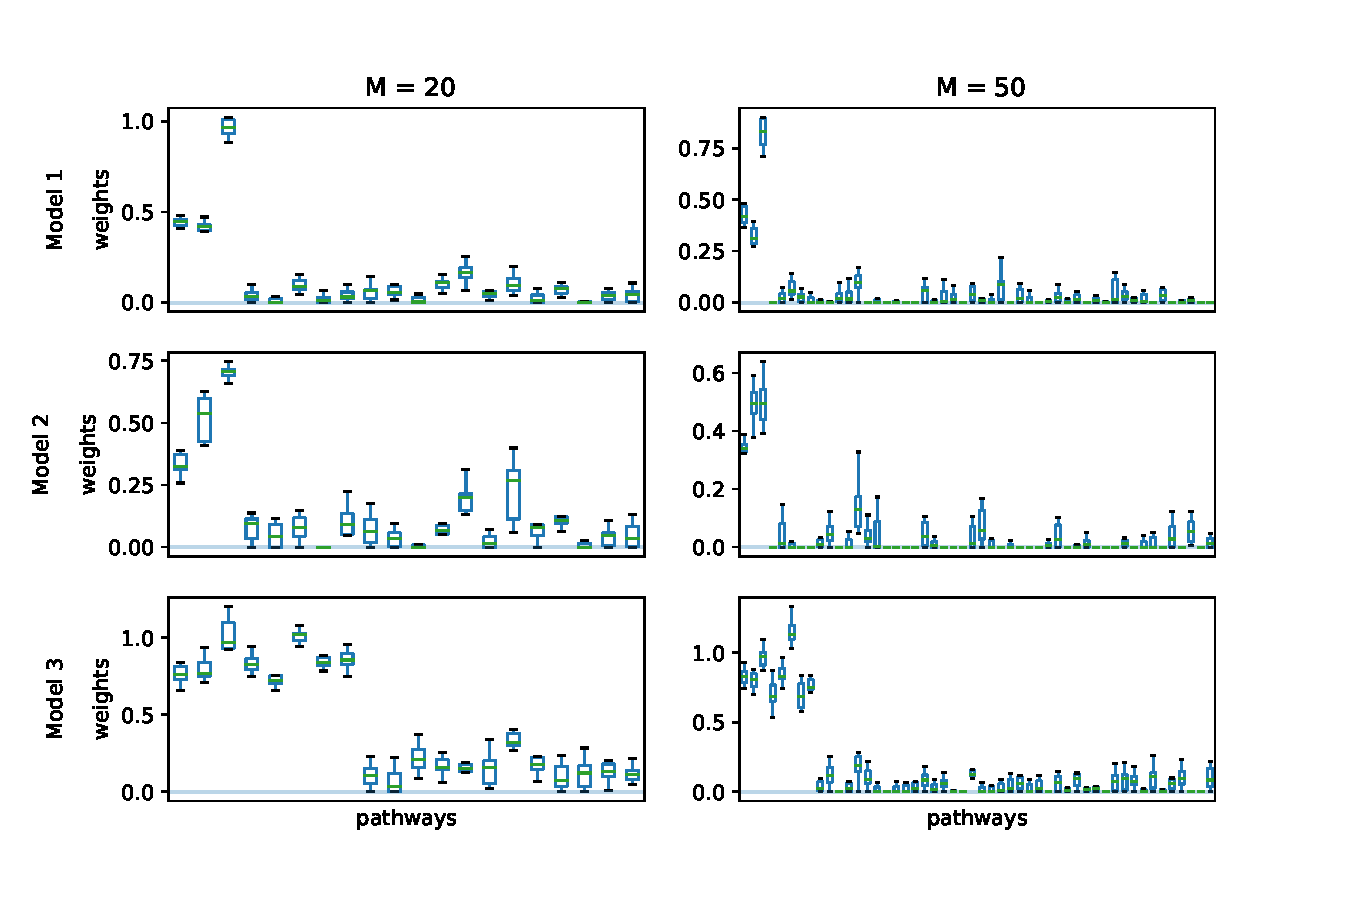
\includegraphics[width=1.07\textwidth]{simu_reg_weights.pdf}
		\caption{Boxplots for pathway weights in the regression simulations. Each box represents the weights distribution for one pathway over ten PKB runs.}
		\label{fig:reg_weights}
	\end{figure}
\newpage
\begin{figure}[h]
	\centering
	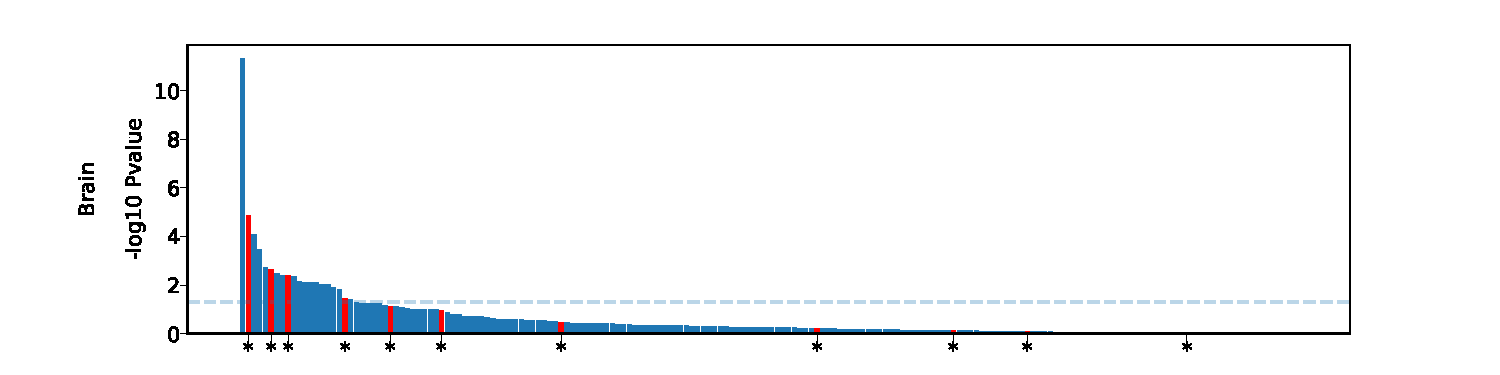
\includegraphics[width=\textwidth]{GSEA_Brain.pdf}\\ \vspace{-3mm}
	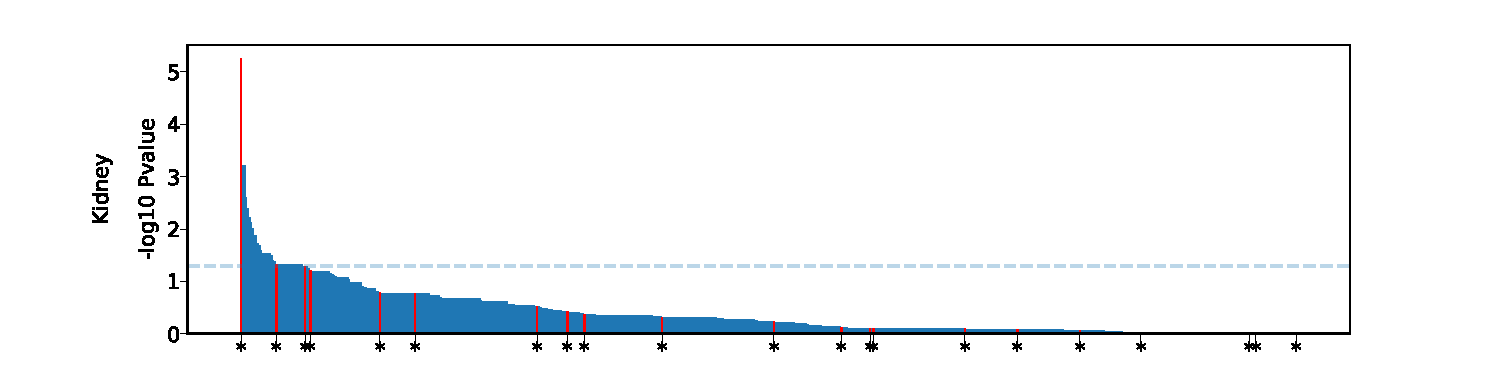
\includegraphics[width=\textwidth]{GSEA_Kidney.pdf}\\ \vspace{-3mm}
	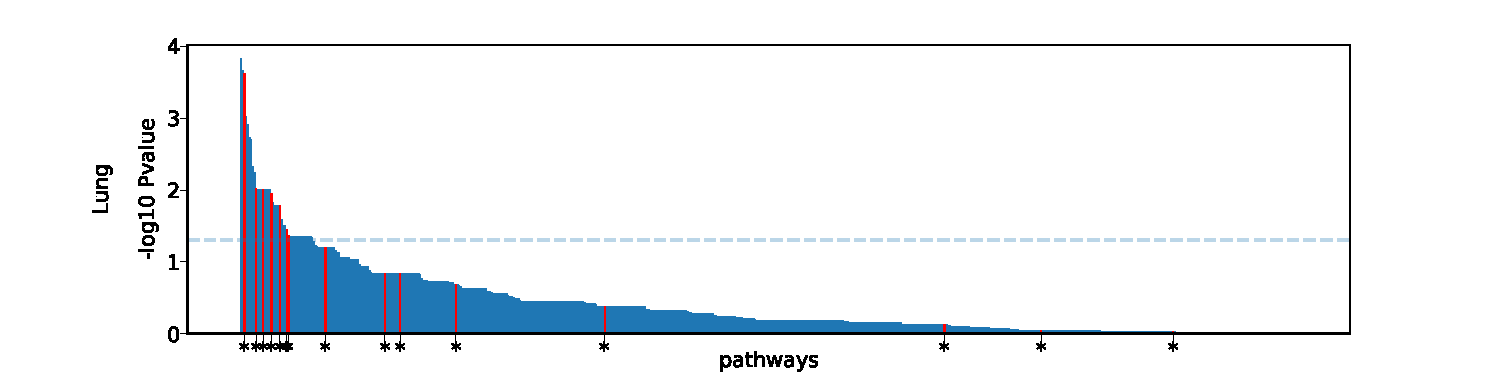
\includegraphics[width=\textwidth]{GSEA_Lung.pdf}
	\caption{Enrichment analysis on brain, kidney, and lung cancer datasets. X-axis represents pathways sorted by their p-values in the enrichment analysis. The blue dashed line corresponds to p-value 0.05. The pathways marked with red bars and stars are pathways with significant weights in PKB.}
	\label{fig:gsea}
\end{figure}
\newpage
\begin{figure}[htp]
	\centering
	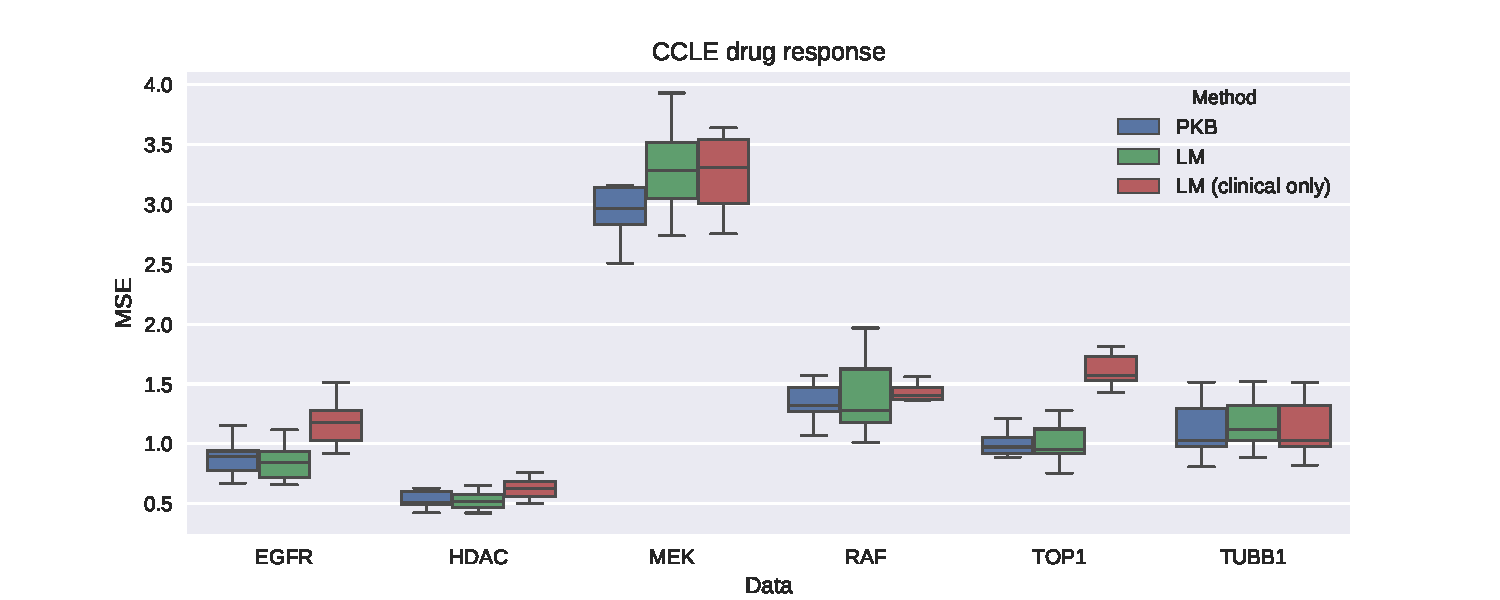
\includegraphics[width = 0.95\textwidth]{PKB_LM_LMc.pdf} \\ \vspace{-4mm}
	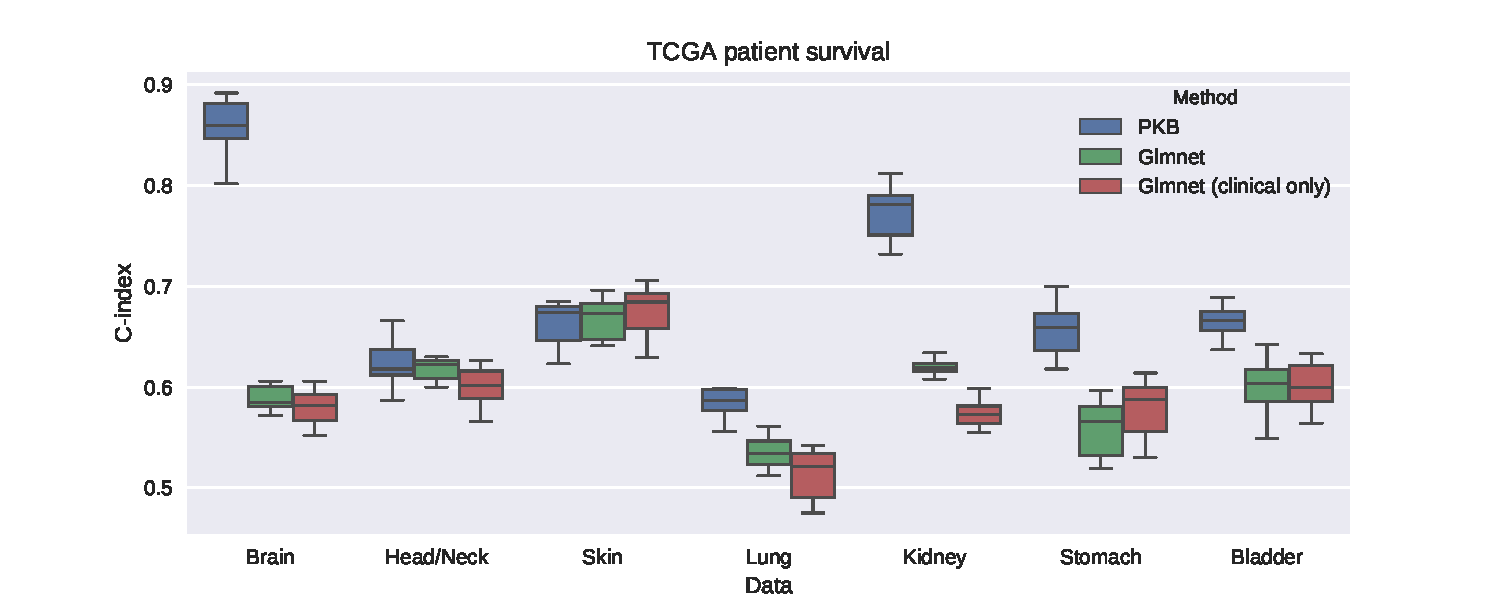
\includegraphics[width = 0.95\textwidth]{PKB_LM_LMc_surv.pdf}
	\caption{Prediction performances from models with and without genomic features. The figure presents the prediction accuracy from three types of models on each dataset. The models include: PKB, linear model, and linear model with only clinical features as predictors. LM in the upper panel represents linear regression model, which reports the best results from LASSO, Ridge Regression, and ElasticNet. The methods with label ``clinical only" are trained without genomic features. The PKB boxes represent the best results from PKB-$L_1$ and PKB-$L_2$.}
	\label{fig:clin_noclin}
\end{figure}
	\newpage
	\begin{table}[htp]
		\centering
		\begin{tabular}{lllllllll}
			\hline
			\multirow{2}{*}{Method} & \multicolumn{2}{c}{Model 1}     &  & \multicolumn{2}{c}{Model 2}     &  & \multicolumn{2}{c}{Model 3}   \\ \cline{2-3} \cline{5-6} \cline{8-9} 
			& M = 20         & M = 50         &  & M = 20         & M = 50         &  & M = 20        & M = 50        \\ \hline
			PKB-$L_1$                  & \textbf{17.11} & \textbf{22.82} &  & \textbf{32.92} & \textbf{33.94} &  & \textbf{7.22} & \textbf{8.37} \\
			PKB-$L_2$                  & \textbf{16.84} & \textbf{22.41} &  & \textbf{31.25} & \textbf{33.65} &  & \textbf{5.4}  & \textbf{5.77} \\
			LASSO                   & 34.85          & 40.58          &  & 49.74          & 50.94          &  & 21.15         & 22.88         \\
			Ridge                   & 50.71          & 53.1           &  & 57.32          & 60.52          &  & 23.25         & 25.99         \\
			ElasticNet              & 34.87          & 42.21          &  & 49.27          & 50.93          &  & 21.25         & 23.51         \\
			RandomForest            & 46.88          & 50.94          &  & 55.34          & 57.34          &  & 21.09         & 22.67         \\
			GBR                     & 48.54          & 51.75          &  & 50.9           & 52.82          &  & 21.46         & 23.7          \\
			SVR                     & 50.02          & 53.58          &  & 56.12          & 59.58          &  & 19.06         & 24.31         \\ \hline
		\end{tabular}
		\caption{Cross-validated MSE of all methods on simulated regression datasets. $M$ represents the number of simulated pathways. For each dataset, MSE values from the top two methods are in boldface.}
		\label{tab:simu_reg}
	\end{table}

\newpage
\begin{table}[htp]
	\centering
	\begin{tabular}{lllllllll}
		\hline
		\multirow{2}{*}{Method} & \multicolumn{2}{c}{Model 1}  & \multicolumn{1}{c}{} & \multicolumn{2}{c}{Model 2}   & \multicolumn{1}{c}{} & \multicolumn{2}{c}{Model 3}   \\ \cline{2-9} 
		& M = 20       & M = 50        &                      & M = 20        & M = 50        &                      & M = 20        & M = 50        \\ \hline
		PKB-$L_1$                  & \textbf{0.9} & \textbf{0.86} & \textbf{}            & \textbf{0.77} & \textbf{0.77} & \textbf{}            & \textbf{0.88} & \textbf{0.87} \\
		PKB-$L_2$                 & \textbf{0.9} & \textbf{0.88} & \textbf{}            & \textbf{0.72} & \textbf{0.76} & \textbf{}            & \textbf{0.9}  & \textbf{0.89} \\
		Glmnet                  & 0.78         & 0.79          &                      & 0.69          & 0.71          &                      & 0.65          & 0.66          \\
		RandomSurvivalForest    & 0.67         & 0.67          &                      & 0.65          & 0.67          &                      & 0.63          & 0.64          \\
		CoxBoost                & 0.78         & 0.78          &                      & 0.7          & 0.7          &                      & 0.66          & 0.66          \\ \hline
	\end{tabular}
	\caption{Cross-validated C-indices of all methods on simulated survival datasets. $M$ represents the number of simulated pathways. For each dataset, C-indices from the top two methods are highlighted in boldface.}
	\label{tab:simu_surv}
\end{table}

\newpage

\begin{table}[htp]
	\centering
	\begin{tabular}{lllllll}
		\hline
		Method       & EGFR          & HDAC          & MEK           & RAF           & TOP1          & TUBB1         \\ \hline
		PKB-$L_1$       & 0.88          & \textbf{0.54} & \textbf{2.92} & \textbf{1.37} & \textbf{0.98} & \textbf{1.12} \\
		PKB-$L_2$       & 0.88          & \textbf{0.54} & \textbf{2.9}  & \textbf{1.35} & 1.01          & \textbf{1.12} \\
		LASSO        & \textbf{0.87} & 0.62          & 3.63          & 1.47          & 1.14          & 1.18          \\
		Ridge        & \textbf{0.84} & \textbf{0.52} & 3.28          & 1.39          & 1.01          & 1.19          \\
		ElasticNet   & 0.89          & 0.59          & 3.37          & 1.44          & 1.14          & 1.17          \\
		RandomForest & 0.88          & 0.56          & 3.17          & \textbf{1.37} & \textbf{0.99} & \textbf{1.12} \\
		GBR          & 0.91          & \textbf{0.54} & 3.3           & 1.43          & 1.0           & 1.14          \\
		SVR          & 0.88          & 0.55          & 3.17          & 1.38          & \textbf{0.99} & \textbf{1.11} \\ \hline
	\end{tabular}
	\caption{Cross-validated MSEs from all methods on CCLE drug response data. For each dataset, the two methods with the smallest MSEs are marked in boldface.}
	\label{tab:ccle_mean}
\end{table}

\newpage

\begin{table}[htp]
	\centering
	\begin{tabular}{llllllll}
		\hline
		Method               & Brain         & Head/Neck          & Skin      & Lung    & Kidney        & Stomach       & Bladder       \\ \hline
		PKB-$L_1$               & \textbf{0.86} & \textbf{0.62} & 0.66          & \textbf{0.59} & \textbf{0.78} & \textbf{0.66} & \textbf{0.67} \\
		PKB-$L_2$               & \textbf{0.85} & 0.61          & 0.64          & \textbf{0.57} & \textbf{0.77} & \textbf{0.65} & \textbf{0.67} \\
		Glmnet               & 0.59          & \textbf{0.62} & \textbf{0.67} & 0.54          & 0.62          & 0.56          & 0.6           \\
		RandomSurvivalForest & 0.58          & 0.54          & 0.63          & 0.54          & 0.58          & 0.54          & 0.52          \\
		CoxBoost             & 0.59          & \textbf{0.62} & \textbf{0.67} & 0.53          & 0.61          & 0.53          & 0.6           \\ \hline
	\end{tabular}
	\caption{Cross-validated C-index from all methods on CCLE drug response data. For each dataset, the two methods with the highest C-index are marked in boldface.}
	\label{tab:tcga_mean}
\end{table}
\end{document}